% Options for packages loaded elsewhere
\PassOptionsToPackage{unicode}{hyperref}
\PassOptionsToPackage{hyphens}{url}
\PassOptionsToPackage{dvipsnames,svgnames,x11names}{xcolor}
%
\documentclass[
  letterpaper,
  DIV=11,
  numbers=noendperiod]{scrreprt}

\usepackage{amsmath,amssymb}
\usepackage{iftex}
\ifPDFTeX
  \usepackage[T1]{fontenc}
  \usepackage[utf8]{inputenc}
  \usepackage{textcomp} % provide euro and other symbols
\else % if luatex or xetex
  \usepackage{unicode-math}
  \defaultfontfeatures{Scale=MatchLowercase}
  \defaultfontfeatures[\rmfamily]{Ligatures=TeX,Scale=1}
\fi
\usepackage{lmodern}
\ifPDFTeX\else  
    % xetex/luatex font selection
\fi
% Use upquote if available, for straight quotes in verbatim environments
\IfFileExists{upquote.sty}{\usepackage{upquote}}{}
\IfFileExists{microtype.sty}{% use microtype if available
  \usepackage[]{microtype}
  \UseMicrotypeSet[protrusion]{basicmath} % disable protrusion for tt fonts
}{}
\makeatletter
\@ifundefined{KOMAClassName}{% if non-KOMA class
  \IfFileExists{parskip.sty}{%
    \usepackage{parskip}
  }{% else
    \setlength{\parindent}{0pt}
    \setlength{\parskip}{6pt plus 2pt minus 1pt}}
}{% if KOMA class
  \KOMAoptions{parskip=half}}
\makeatother
\usepackage{xcolor}
\setlength{\emergencystretch}{3em} % prevent overfull lines
\setcounter{secnumdepth}{5}
% Make \paragraph and \subparagraph free-standing
\makeatletter
\ifx\paragraph\undefined\else
  \let\oldparagraph\paragraph
  \renewcommand{\paragraph}{
    \@ifstar
      \xxxParagraphStar
      \xxxParagraphNoStar
  }
  \newcommand{\xxxParagraphStar}[1]{\oldparagraph*{#1}\mbox{}}
  \newcommand{\xxxParagraphNoStar}[1]{\oldparagraph{#1}\mbox{}}
\fi
\ifx\subparagraph\undefined\else
  \let\oldsubparagraph\subparagraph
  \renewcommand{\subparagraph}{
    \@ifstar
      \xxxSubParagraphStar
      \xxxSubParagraphNoStar
  }
  \newcommand{\xxxSubParagraphStar}[1]{\oldsubparagraph*{#1}\mbox{}}
  \newcommand{\xxxSubParagraphNoStar}[1]{\oldsubparagraph{#1}\mbox{}}
\fi
\makeatother

\usepackage{color}
\usepackage{fancyvrb}
\newcommand{\VerbBar}{|}
\newcommand{\VERB}{\Verb[commandchars=\\\{\}]}
\DefineVerbatimEnvironment{Highlighting}{Verbatim}{commandchars=\\\{\}}
% Add ',fontsize=\small' for more characters per line
\usepackage{framed}
\definecolor{shadecolor}{RGB}{241,243,245}
\newenvironment{Shaded}{\begin{snugshade}}{\end{snugshade}}
\newcommand{\AlertTok}[1]{\textcolor[rgb]{0.68,0.00,0.00}{#1}}
\newcommand{\AnnotationTok}[1]{\textcolor[rgb]{0.37,0.37,0.37}{#1}}
\newcommand{\AttributeTok}[1]{\textcolor[rgb]{0.40,0.45,0.13}{#1}}
\newcommand{\BaseNTok}[1]{\textcolor[rgb]{0.68,0.00,0.00}{#1}}
\newcommand{\BuiltInTok}[1]{\textcolor[rgb]{0.00,0.23,0.31}{#1}}
\newcommand{\CharTok}[1]{\textcolor[rgb]{0.13,0.47,0.30}{#1}}
\newcommand{\CommentTok}[1]{\textcolor[rgb]{0.37,0.37,0.37}{#1}}
\newcommand{\CommentVarTok}[1]{\textcolor[rgb]{0.37,0.37,0.37}{\textit{#1}}}
\newcommand{\ConstantTok}[1]{\textcolor[rgb]{0.56,0.35,0.01}{#1}}
\newcommand{\ControlFlowTok}[1]{\textcolor[rgb]{0.00,0.23,0.31}{\textbf{#1}}}
\newcommand{\DataTypeTok}[1]{\textcolor[rgb]{0.68,0.00,0.00}{#1}}
\newcommand{\DecValTok}[1]{\textcolor[rgb]{0.68,0.00,0.00}{#1}}
\newcommand{\DocumentationTok}[1]{\textcolor[rgb]{0.37,0.37,0.37}{\textit{#1}}}
\newcommand{\ErrorTok}[1]{\textcolor[rgb]{0.68,0.00,0.00}{#1}}
\newcommand{\ExtensionTok}[1]{\textcolor[rgb]{0.00,0.23,0.31}{#1}}
\newcommand{\FloatTok}[1]{\textcolor[rgb]{0.68,0.00,0.00}{#1}}
\newcommand{\FunctionTok}[1]{\textcolor[rgb]{0.28,0.35,0.67}{#1}}
\newcommand{\ImportTok}[1]{\textcolor[rgb]{0.00,0.46,0.62}{#1}}
\newcommand{\InformationTok}[1]{\textcolor[rgb]{0.37,0.37,0.37}{#1}}
\newcommand{\KeywordTok}[1]{\textcolor[rgb]{0.00,0.23,0.31}{\textbf{#1}}}
\newcommand{\NormalTok}[1]{\textcolor[rgb]{0.00,0.23,0.31}{#1}}
\newcommand{\OperatorTok}[1]{\textcolor[rgb]{0.37,0.37,0.37}{#1}}
\newcommand{\OtherTok}[1]{\textcolor[rgb]{0.00,0.23,0.31}{#1}}
\newcommand{\PreprocessorTok}[1]{\textcolor[rgb]{0.68,0.00,0.00}{#1}}
\newcommand{\RegionMarkerTok}[1]{\textcolor[rgb]{0.00,0.23,0.31}{#1}}
\newcommand{\SpecialCharTok}[1]{\textcolor[rgb]{0.37,0.37,0.37}{#1}}
\newcommand{\SpecialStringTok}[1]{\textcolor[rgb]{0.13,0.47,0.30}{#1}}
\newcommand{\StringTok}[1]{\textcolor[rgb]{0.13,0.47,0.30}{#1}}
\newcommand{\VariableTok}[1]{\textcolor[rgb]{0.07,0.07,0.07}{#1}}
\newcommand{\VerbatimStringTok}[1]{\textcolor[rgb]{0.13,0.47,0.30}{#1}}
\newcommand{\WarningTok}[1]{\textcolor[rgb]{0.37,0.37,0.37}{\textit{#1}}}

\providecommand{\tightlist}{%
  \setlength{\itemsep}{0pt}\setlength{\parskip}{0pt}}\usepackage{longtable,booktabs,array}
\usepackage{calc} % for calculating minipage widths
% Correct order of tables after \paragraph or \subparagraph
\usepackage{etoolbox}
\makeatletter
\patchcmd\longtable{\par}{\if@noskipsec\mbox{}\fi\par}{}{}
\makeatother
% Allow footnotes in longtable head/foot
\IfFileExists{footnotehyper.sty}{\usepackage{footnotehyper}}{\usepackage{footnote}}
\makesavenoteenv{longtable}
\usepackage{graphicx}
\makeatletter
\def\maxwidth{\ifdim\Gin@nat@width>\linewidth\linewidth\else\Gin@nat@width\fi}
\def\maxheight{\ifdim\Gin@nat@height>\textheight\textheight\else\Gin@nat@height\fi}
\makeatother
% Scale images if necessary, so that they will not overflow the page
% margins by default, and it is still possible to overwrite the defaults
% using explicit options in \includegraphics[width, height, ...]{}
\setkeys{Gin}{width=\maxwidth,height=\maxheight,keepaspectratio}
% Set default figure placement to htbp
\makeatletter
\def\fps@figure{htbp}
\makeatother
% definitions for citeproc citations
\NewDocumentCommand\citeproctext{}{}
\NewDocumentCommand\citeproc{mm}{%
  \begingroup\def\citeproctext{#2}\cite{#1}\endgroup}
\makeatletter
 % allow citations to break across lines
 \let\@cite@ofmt\@firstofone
 % avoid brackets around text for \cite:
 \def\@biblabel#1{}
 \def\@cite#1#2{{#1\if@tempswa , #2\fi}}
\makeatother
\newlength{\cslhangindent}
\setlength{\cslhangindent}{1.5em}
\newlength{\csllabelwidth}
\setlength{\csllabelwidth}{3em}
\newenvironment{CSLReferences}[2] % #1 hanging-indent, #2 entry-spacing
 {\begin{list}{}{%
  \setlength{\itemindent}{0pt}
  \setlength{\leftmargin}{0pt}
  \setlength{\parsep}{0pt}
  % turn on hanging indent if param 1 is 1
  \ifodd #1
   \setlength{\leftmargin}{\cslhangindent}
   \setlength{\itemindent}{-1\cslhangindent}
  \fi
  % set entry spacing
  \setlength{\itemsep}{#2\baselineskip}}}
 {\end{list}}
\usepackage{calc}
\newcommand{\CSLBlock}[1]{\hfill\break\parbox[t]{\linewidth}{\strut\ignorespaces#1\strut}}
\newcommand{\CSLLeftMargin}[1]{\parbox[t]{\csllabelwidth}{\strut#1\strut}}
\newcommand{\CSLRightInline}[1]{\parbox[t]{\linewidth - \csllabelwidth}{\strut#1\strut}}
\newcommand{\CSLIndent}[1]{\hspace{\cslhangindent}#1}

\KOMAoption{captions}{tableheading}
\makeatletter
\@ifpackageloaded{bookmark}{}{\usepackage{bookmark}}
\makeatother
\makeatletter
\@ifpackageloaded{caption}{}{\usepackage{caption}}
\AtBeginDocument{%
\ifdefined\contentsname
  \renewcommand*\contentsname{Table of contents}
\else
  \newcommand\contentsname{Table of contents}
\fi
\ifdefined\listfigurename
  \renewcommand*\listfigurename{List of Figures}
\else
  \newcommand\listfigurename{List of Figures}
\fi
\ifdefined\listtablename
  \renewcommand*\listtablename{List of Tables}
\else
  \newcommand\listtablename{List of Tables}
\fi
\ifdefined\figurename
  \renewcommand*\figurename{Figure}
\else
  \newcommand\figurename{Figure}
\fi
\ifdefined\tablename
  \renewcommand*\tablename{Table}
\else
  \newcommand\tablename{Table}
\fi
}
\@ifpackageloaded{float}{}{\usepackage{float}}
\floatstyle{ruled}
\@ifundefined{c@chapter}{\newfloat{codelisting}{h}{lop}}{\newfloat{codelisting}{h}{lop}[chapter]}
\floatname{codelisting}{Listing}
\newcommand*\listoflistings{\listof{codelisting}{List of Listings}}
\makeatother
\makeatletter
\makeatother
\makeatletter
\@ifpackageloaded{caption}{}{\usepackage{caption}}
\@ifpackageloaded{subcaption}{}{\usepackage{subcaption}}
\makeatother

\ifLuaTeX
  \usepackage{selnolig}  % disable illegal ligatures
\fi
\usepackage{bookmark}

\IfFileExists{xurl.sty}{\usepackage{xurl}}{} % add URL line breaks if available
\urlstyle{same} % disable monospaced font for URLs
\hypersetup{
  pdftitle={Biology 305: Biostatistics},
  pdfauthor={Dr.~Jacob C. Cooper \& Dr.~Melissa Wuellner},
  colorlinks=true,
  linkcolor={blue},
  filecolor={Maroon},
  citecolor={Blue},
  urlcolor={Blue},
  pdfcreator={LaTeX via pandoc}}


\title{Biology 305: Biostatistics}
\author{Dr.~Jacob C. Cooper \& Dr.~Melissa Wuellner}
\date{Invalid Date}

\begin{document}
\maketitle

\renewcommand*\contentsname{Table of contents}
{
\hypersetup{linkcolor=}
\setcounter{tocdepth}{2}
\tableofcontents
}

\bookmarksetup{startatroot}

\chapter*{Preface}\label{preface}
\addcontentsline{toc}{chapter}{Preface}

\markboth{Preface}{Preface}

Welcome to Biology 105 at the University of Nebraska at Kearney!
Material in this class was designed by Dr.~Melissa Wuellner and adapted
by Dr.~Jacob C. Cooper for use in \emph{R}.

In this class, you will learn:

\begin{enumerate}
\def\labelenumi{\arabic{enumi}.}
\tightlist
\item
  The basics of study design, the importance of understanding your
  research situation before embarking on a full study, and practice
  creating research frameworks based on different scenarios.
\item
  The basics of data analysis, including understanding what kind of
  variables are being collected, why understanding variable types are
  important, and basic tests to understand univariate distributions.
\item
  Basic multivariate statistics, including ANOVA, correlation, and
  regression, for comparing multiple different groups.
\item
  The basics of coding and working in \emph{R} for performing
  statistical analyses.
\end{enumerate}

This site will help you navigate different homework assignments to
perform the necessary \emph{R} tests. Furthermore, this GitHub
repository contains all of the homework dataframes, so you will
\emph{not} have to manually enter assignments if you use \emph{R} to
complete your assignments.

Welcome to class!

Dr.~Jacob C. Cooper, BHS 321

\bookmarksetup{startatroot}

\chapter{\texorpdfstring{Intro to
\emph{R}}{Intro to R}}\label{intro-to-r}

In this class, we will be using \emph{R} to perform statistical
analyses. \emph{R} is a free software program designed for use in a
myriad of statistical and computational scenarios. It can handle
extremely large datasets, can handle spatial data, and has wrappers for
compatibility with \emph{Python}, \emph{Bash}, and other programs (even
\emph{Java}!).

\bookmarksetup{startatroot}

\chapter{Setup}\label{setup}

First, we need to download \emph{R} onto your machine. We are also going
to download \emph{RStudio} to assist with creating \emph{R} scripts and
documents.

\section{\texorpdfstring{Installing
\emph{R}}{Installing R}}\label{installing-r}

First, navigate to the \href{https://cloud.r-project.org/}{\emph{R}
download and install page}. Download the appropriate version for your
operating system (Windows, Mac, or Linux). \textbf{Note} that coding
will be formatted slightly different for Windows than for other
operating systems.

Follow the installation steps for \emph{R}, and verify that the
installation was successful by searching for \emph{R} on your machine.
You should be presented with a coding window that looks like the
following:

\begin{verbatim}
R version 4.4.1 (2024-06-14) -- "Race for Your Life"
Copyright (C) 2024 The R Foundation for Statistical Computing
Platform: aarch64-apple-darwin20

R is free software and comes with ABSOLUTELY NO WARRANTY.
You are welcome to redistribute it under certain conditions.
Type 'license()' or 'licence()' for distribution details.

  Natural language support but running in an English locale

R is a collaborative project with many contributors.
Type 'contributors()' for more information and
'citation()' on how to cite R or R packages in publications.

Type 'demo()' for some demos, 'help()' for on-line help, or
'help.start()' for an HTML browser interface to help.
Type 'q()' to quit R.

>
\end{verbatim}

If that screen appears, congratulations! \emph{R} is properly installed.
If the install was not successful, please talk to Dr.~Cooper and check
with your classmates as well.

\section{\texorpdfstring{Installing
\emph{RStudio}}{Installing RStudio}}\label{installing-rstudio}

\emph{RStudio} is a GUI (graphics user interface) that helps make
\emph{R} easier to use. Furthermore, it allows you to create documents
in \emph{R}, including websites (such as this one), PDFs, and even
presentations. This can greatly streamline the research pipeline and
help you publish your results and associated code in a quick and
efficient fashion.

Head over the the \href{https://posit.co/downloads/}{\emph{RStudio}
download website} and download ``\emph{RStudio} Desktop'', which is
free. Be sure to pick the correct version for your machine.

Open \emph{RStudio} on your machine. You should be presented with
something like the following:

\begin{figure}[H]

{\centering 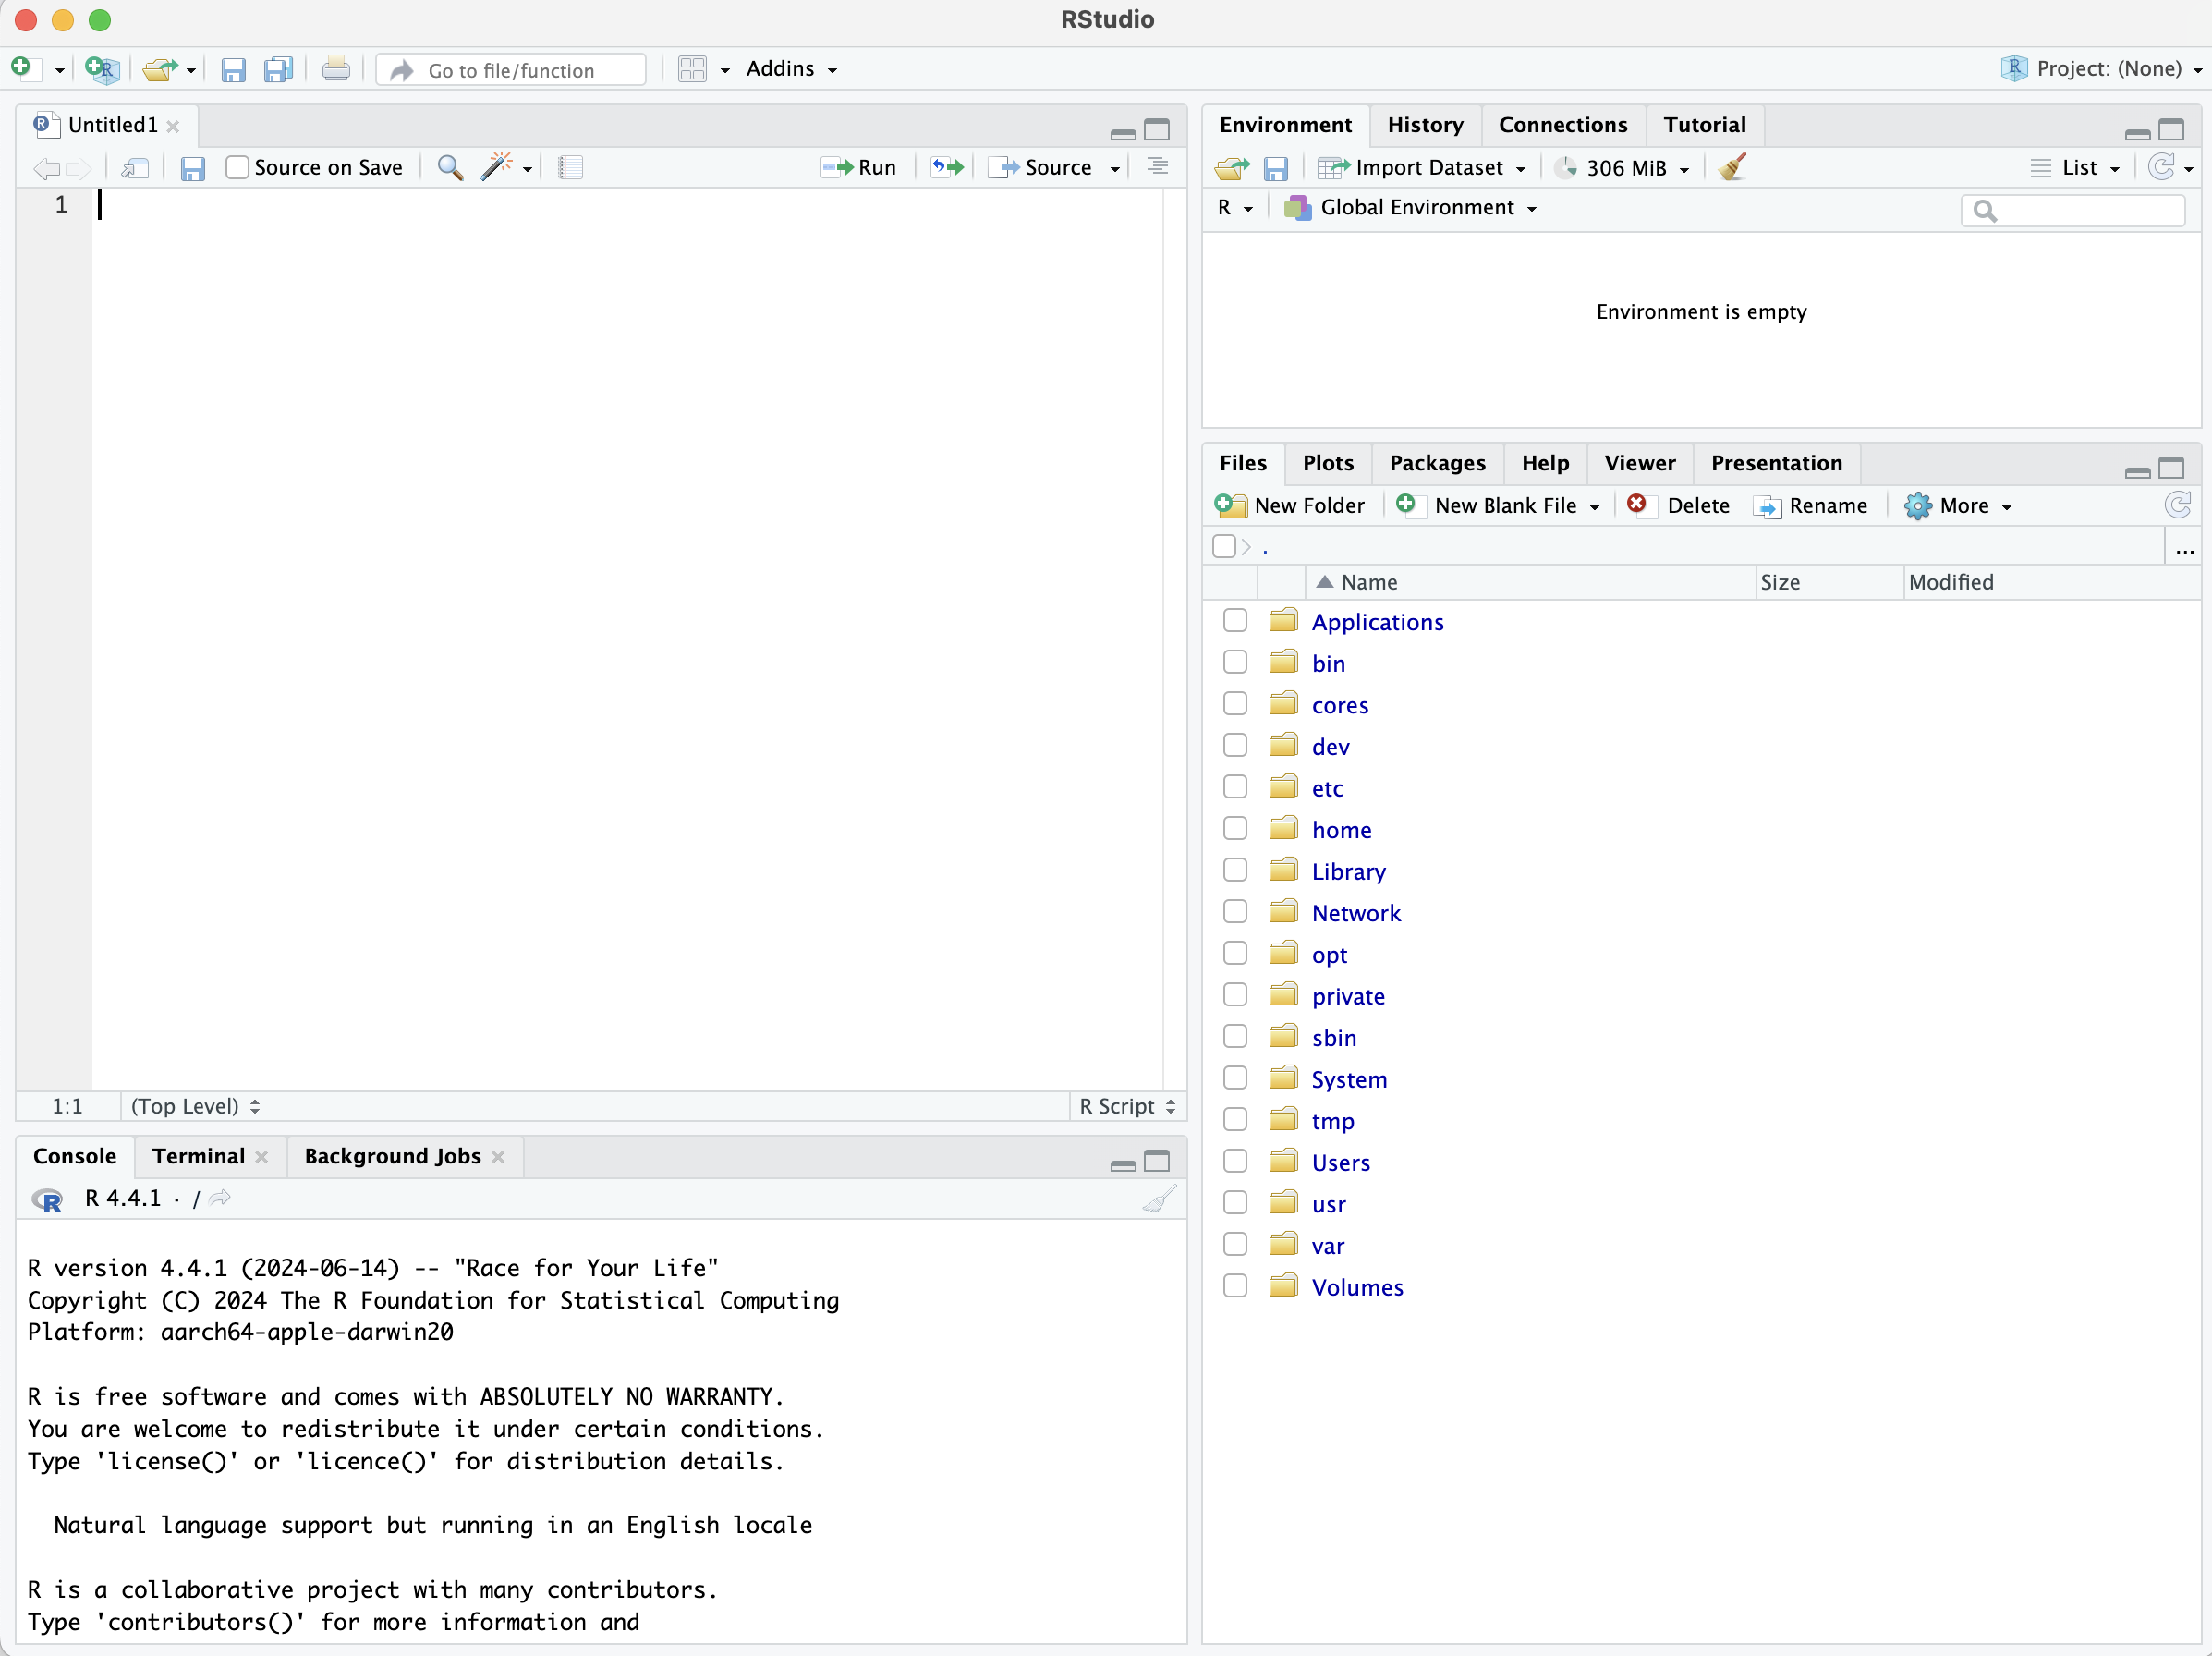
\includegraphics{images/rstudio_start.png}

}

\caption{\emph{RStudio} start window. Note that the screen is split into
four different quadrants. Top left: \emph{R} documents; bottom left:
\emph{R} program; top right: environment window; bottom right: plots,
help, and directories.}

\end{figure}%

In \emph{RStudio}, the top left window is always going to be our coding
window. This is where we will type all of our code and create our
documents. In the bottom left we will see \emph{R} executing the code.
This will show what the computer is ``thinking'' and will help us spot
any potential issues. The top right window is the ``environment'', which
shows what variables and datasets are stored within the computers'
memory. (It can also show some other things, but we aren't concerned
with that at this point). The bottom right window is the ``display''
window. This is where plots and help windows will appear if they don't
appear in the document (top left) window itself.

Now, we will create our first \emph{R} document!

\bookmarksetup{startatroot}

\chapter{\texorpdfstring{Creating an \emph{RMarkdown}
document}{Creating an RMarkdown document}}\label{creating-an-rmarkdown-document}

\section{Setup}\label{setup-1}

In this class, we will be creating assignments in what is called
\emph{RMarkdown}. This is a rich-text version of \emph{R} that allows us
to create documents with the code embedded. In \emph{RStudio}, click the
``+'' button in the far top left to open the \texttt{New\ Document}
menu. Scroll down this list and click on \texttt{R\ Markdown}.

A screen such as this will appear:

\begin{figure}[H]

{\centering 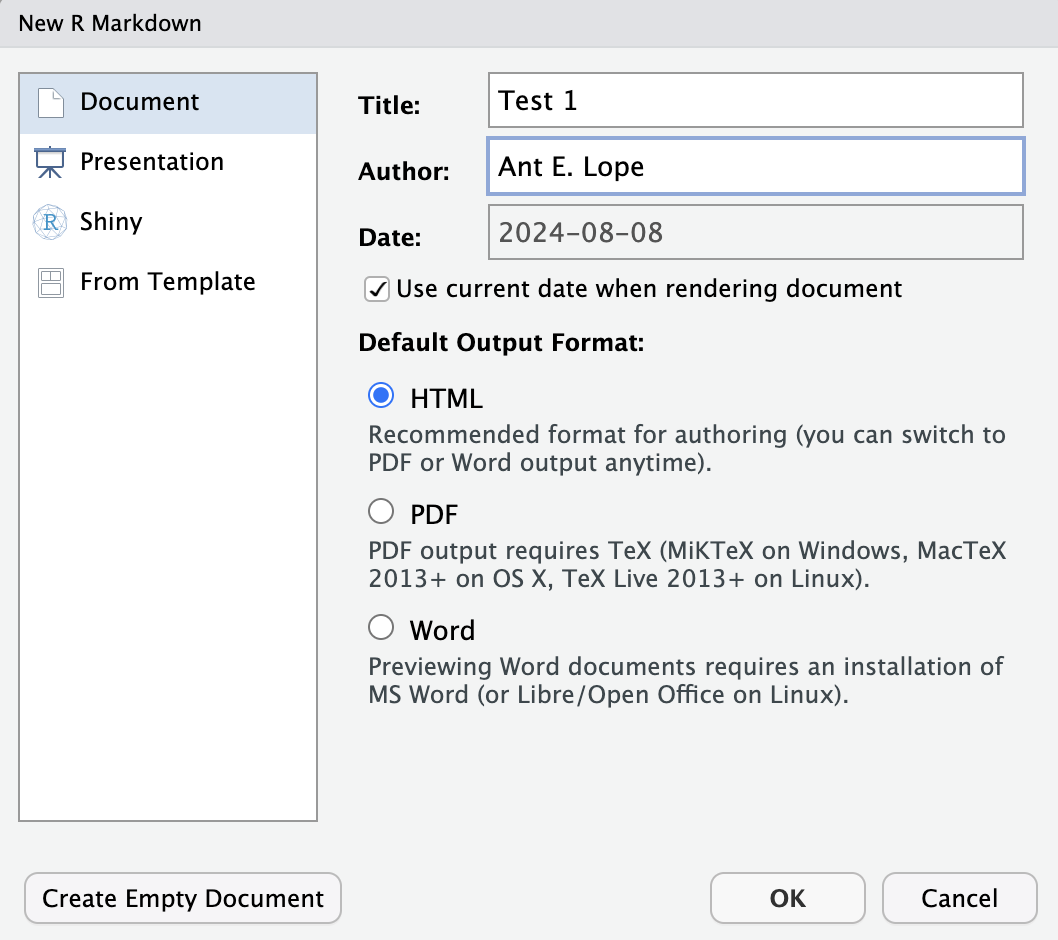
\includegraphics{images/newfile.png}

}

\caption{A new file window for an \emph{RMarkdown} file.}

\end{figure}%

After entering a title and your name and selecting \texttt{document} in
the left hand menu, click \texttt{OK}.

\begin{figure}[H]

{\centering 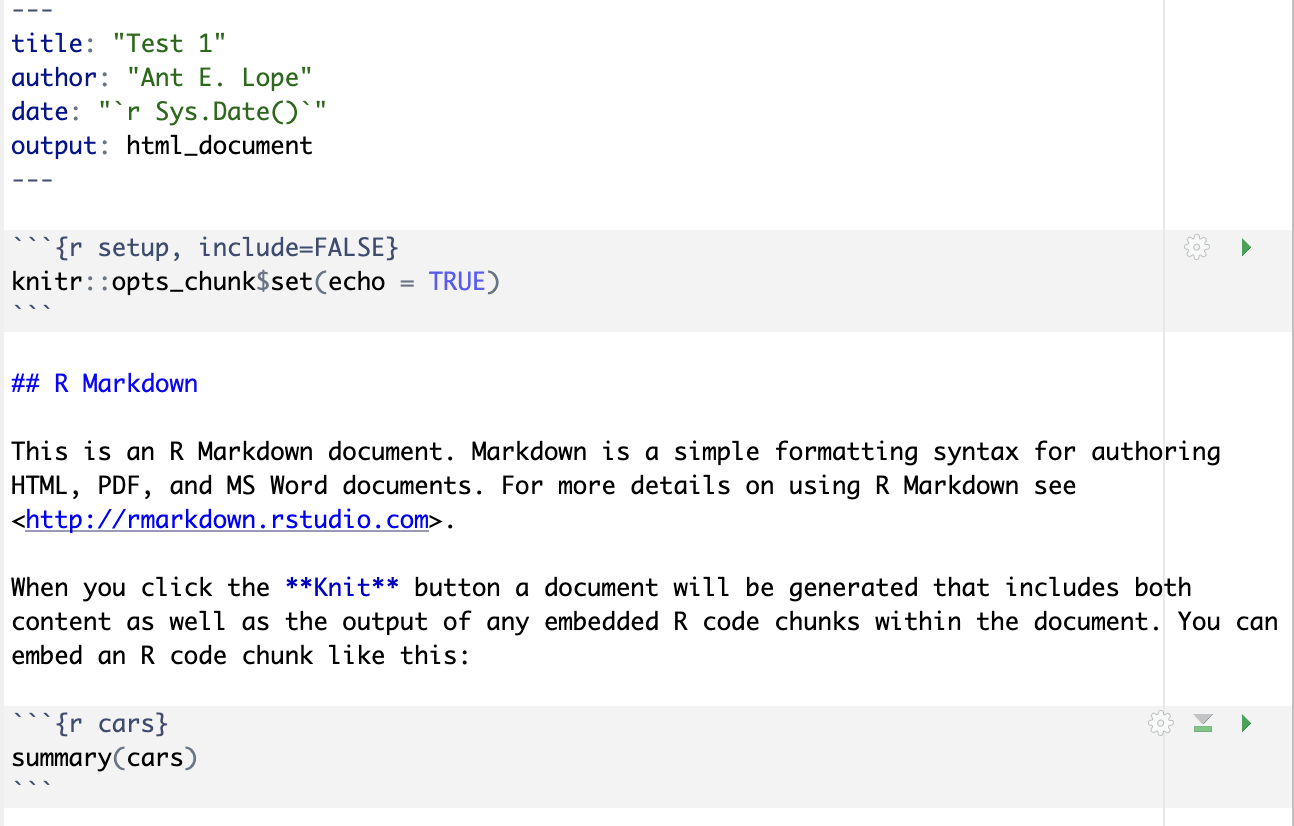
\includegraphics{images/markdown.png}

}

\caption{An example of a markdown script.}

\end{figure}%

In the image above, we can see what a ``default'' \emph{RMarkdown}
script looks like after creating the file. At the top of the document,
between all of the dashes, we have the \texttt{yaml} header that tells
\emph{R} what kind of document will be created, who the author is, and
tells it to use today's date. In this class, we will be saving documents
as \texttt{html} as they are the easiest documents to create and save.
These documents will include all of your code, text, and even any plots
you may create!

Plain text in the document will be rendered as plain text in the
document. (I.e., whatever you type normally will become ``normal text''
in the finished document). Lines preceded with \texttt{\#} will become
headers, with \texttt{\#\#} being a second level header and
\texttt{\#\#\#} being a third level header, etc. Words can also be made
italic by putting an asterisk on each side of the word
(\texttt{*italic*}) and bold by putting two asterisks on each side
(\texttt{**bold**}). URLs are also supported, with
\texttt{\textless{}\textgreater{}} on each side of a URL making it
clickable, and words being hyperlinked by typing
\texttt{{[}words\ to\ show{]}(target\ URL)}.

We also have code ``chunks'' that are shown above. A code chunk can be
manually typed out or inserted by pressing \texttt{CTRL} + \texttt{ALT}
+ \texttt{I} (Windows, Linux) or \texttt{COMMAND} + \texttt{OPTION} +
\texttt{I} (Mac). Everything inside a ``code chunk'' will be read as
\emph{R} code and executed as such. Note that you can have additional
commands in the \emph{R} chunks, but we won't cover that for now.

\section{Using code chunks}\label{using-code-chunks}

In your computer, erase all information except for the \texttt{yaml}
header between the dashes on your computer. \texttt{Save} your file in a
folder where you want your assignment to be located. It is important you
do this step up front as the computer will sometimes save in random
places if you don't specify a file location at the beginning.
\emph{Don't forget to save your work frequently}!

\begin{figure}[H]

{\centering 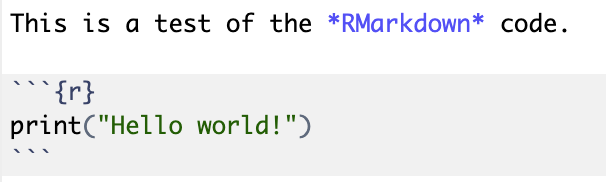
\includegraphics{images/test_text.png}

}

\caption{Text to type in your \emph{Rmarkdown} document.}

\end{figure}%

After typing this into the document, hit \texttt{knit} near the top of
the upper left window. \emph{R} will now create an HTML document that
should look like this:

\begin{figure}[H]

{\centering 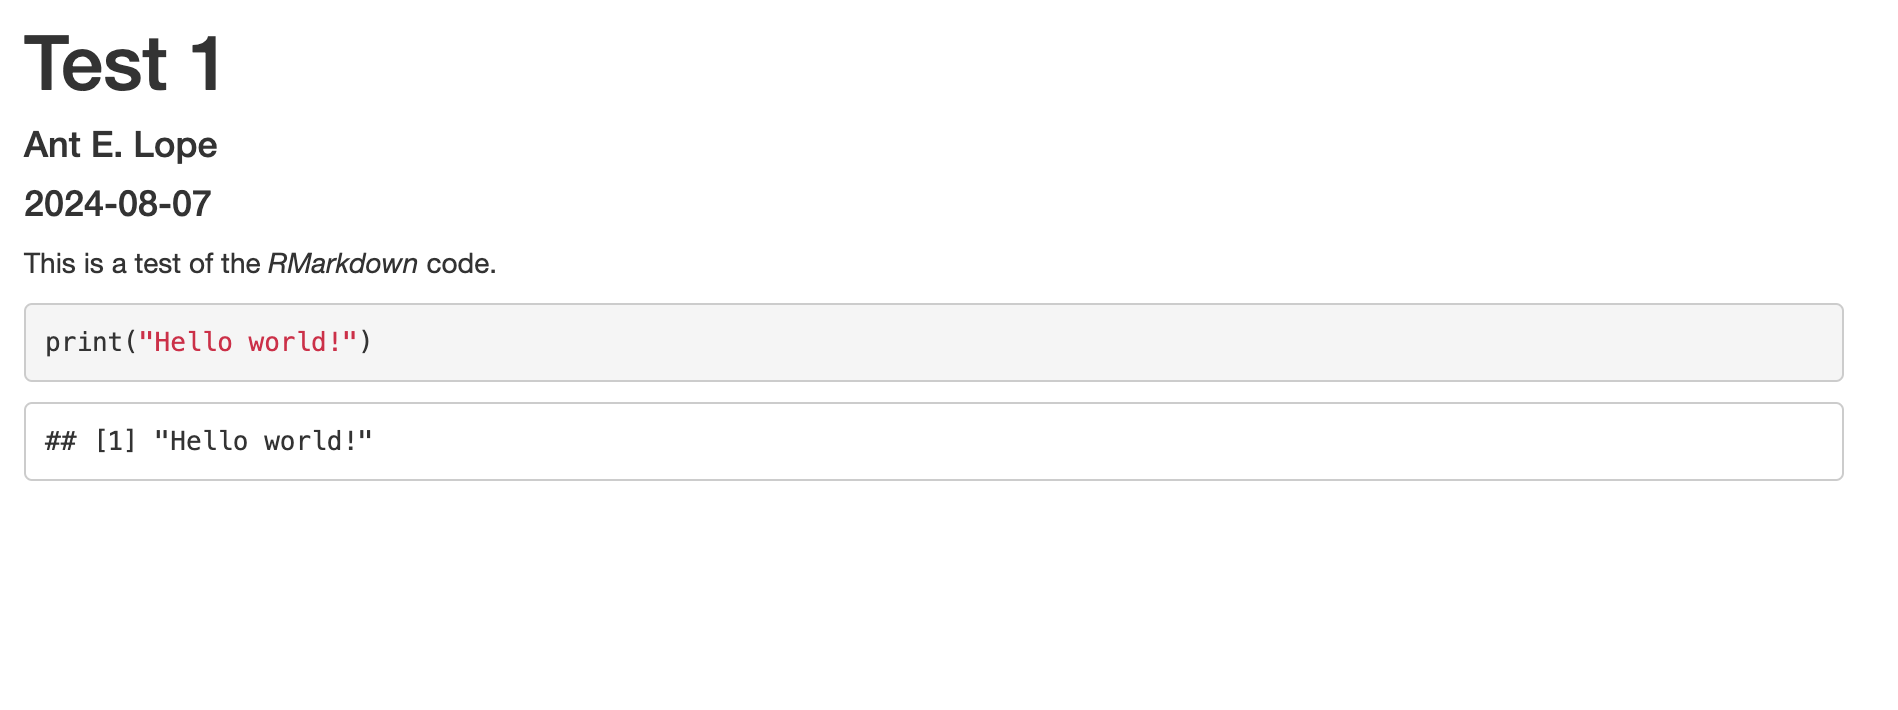
\includegraphics{images/test1.png}

}

\caption{The output from the above code knitted into a document.}

\end{figure}%

We can see now that the \texttt{HTML} document has the title of the
document, the author's name, the date on which the code was run, and a
greyed-out box with color coded \emph{R} code followed by the output.
Let's try something a little more complex. Create a new code chunk and
type the following:

\begin{Shaded}
\begin{Highlighting}[]
\NormalTok{x }\OtherTok{\textless{}{-}} \DecValTok{1}\SpecialCharTok{:}\DecValTok{10}
\end{Highlighting}
\end{Shaded}

This will create a variable in \emph{R}, \texttt{x}, that is
sequentially each whole number between 1 and 10. We can see this by
highlighting or typing only the letter \texttt{x} and running that line
of code by clicking \texttt{CTRL} + \texttt{ENTER} (Windows / Linux) or
\texttt{COMMAND} + \texttt{ENTER} (Mac).

\begin{Shaded}
\begin{Highlighting}[]
\NormalTok{x}
\end{Highlighting}
\end{Shaded}

\begin{verbatim}
 [1]  1  2  3  4  5  6  7  8  9 10
\end{verbatim}

If you look at the top right window, you will also see the value
\texttt{x} in the environment defined as
\texttt{int\ {[}1:10{]}\ 1\ 2\ 3\ 4\ 5\ 6\ 7\ 8\ 9\ 10}. This indicates
that \texttt{x} is integer data spanning ten positions numbered 1 to 10.
Since the vector is small, it displays every number in the sequence.

\begin{figure}[H]

{\centering 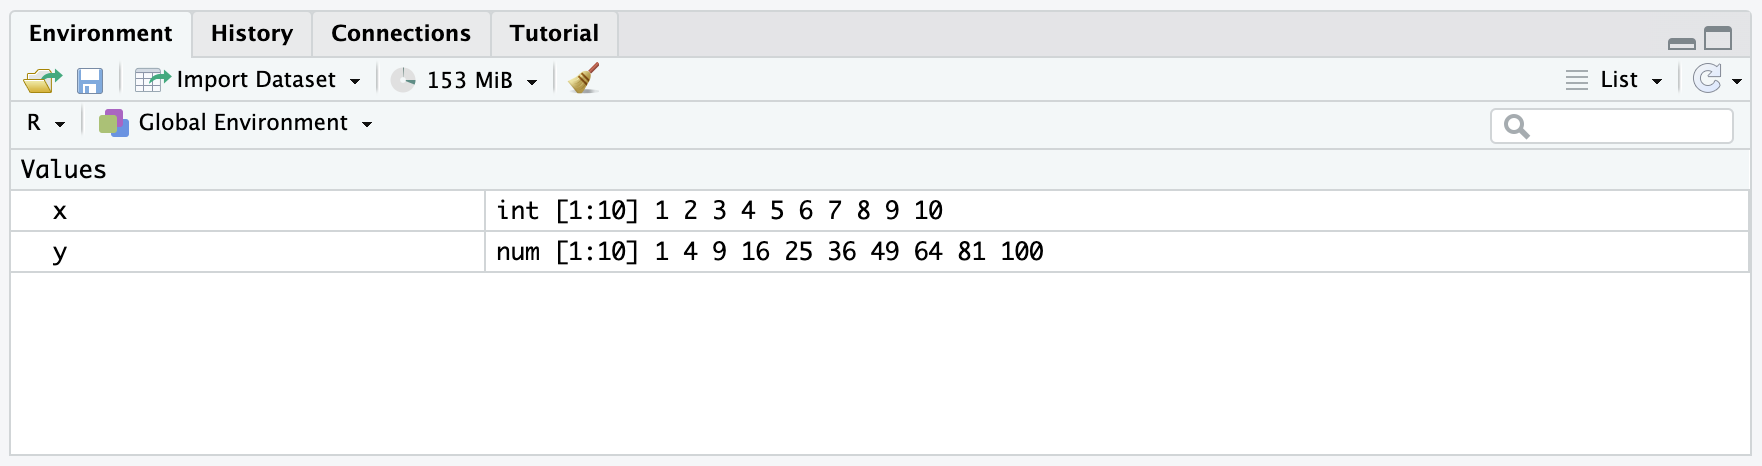
\includegraphics{images/environment.png}

}

\caption{\emph{RStudio} environment window showing saved objects. These
are in the computer's memory.}

\end{figure}%

Let's create another vector \texttt{y} that is the squared values of
\texttt{x}, such that \(y=x^2\). We can raise values to an exponent by
using \texttt{\^{}}.

\begin{Shaded}
\begin{Highlighting}[]
\NormalTok{y }\OtherTok{\textless{}{-}}\NormalTok{ x}\SpecialCharTok{\^{}}\DecValTok{2}
\NormalTok{y}
\end{Highlighting}
\end{Shaded}

\begin{verbatim}
 [1]   1   4   9  16  25  36  49  64  81 100
\end{verbatim}

Now we have the value \texttt{y} in the environment that is the square
of the values of \texttt{x}. This is a \texttt{numeric} vector of 10
values numbered 1 to 10 where each value corresponds to a square of the
\texttt{x} value. We can raise things to any value however, including
\(x^x\)!

\begin{Shaded}
\begin{Highlighting}[]
\NormalTok{x}\SpecialCharTok{\^{}}\NormalTok{x}
\end{Highlighting}
\end{Shaded}

\begin{verbatim}
 [1]           1           4          27         256        3125       46656
 [7]      823543    16777216   387420489 10000000000
\end{verbatim}

As we can see, since I didn't ``store'' this value as a variable in
\emph{R} using \texttt{\textless{}-}, the value is not in the
environment.

\section{Plotting}\label{plotting}

Now, let's try creating a plot. This is easy in \emph{R}, as we just use
the command \texttt{plot}.

\begin{Shaded}
\begin{Highlighting}[]
\FunctionTok{plot}\NormalTok{(}\AttributeTok{x =}\NormalTok{ x, }\AttributeTok{y =}\NormalTok{ y)}
\end{Highlighting}
\end{Shaded}

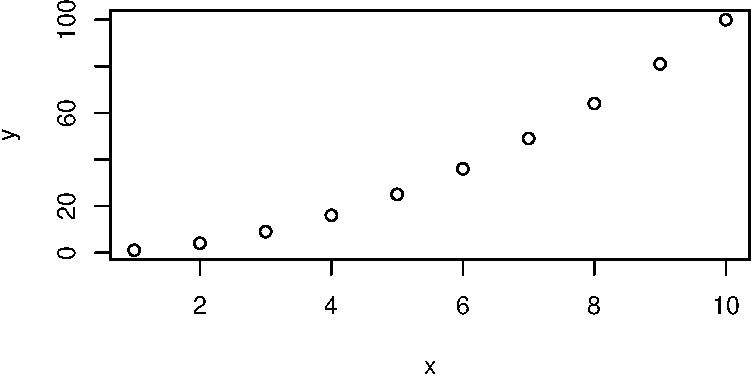
\includegraphics{intro_to_r_files/figure-pdf/unnamed-chunk-5-1.pdf}

By specifying the \texttt{y} and \texttt{x} components in \texttt{plot},
we can quickly generate a point plot. We can alter the visual parameters
of this plot using a few different commands. I will outline these below
with inline notes. Inline notes in the code can be made by using a
\texttt{\#} symbol before them, which basically tells \emph{R} to ignore
everything after the \texttt{\#}. For example:

\begin{Shaded}
\begin{Highlighting}[]
\FunctionTok{print}\NormalTok{(}\StringTok{"Test"}\NormalTok{)}
\end{Highlighting}
\end{Shaded}

\begin{verbatim}
[1] "Test"
\end{verbatim}

\begin{Shaded}
\begin{Highlighting}[]
\CommentTok{\# print("Test 2")}
\end{Highlighting}
\end{Shaded}

This prints the word \texttt{Test}, but doesn't print \texttt{Test\ 2}.

Now let's make the plot with some new visual parameters.

\begin{Shaded}
\begin{Highlighting}[]
\FunctionTok{plot}\NormalTok{(}\AttributeTok{x =}\NormalTok{ x, }\CommentTok{\# specify x values}
     \AttributeTok{y =}\NormalTok{ y, }\CommentTok{\# specify y values}
     \AttributeTok{ylab =} \StringTok{"Y Values"}\NormalTok{, }\CommentTok{\# specify Y label}
     \AttributeTok{xlab =} \StringTok{"X Values"}\NormalTok{, }\CommentTok{\# specify X label}
     \AttributeTok{main =} \StringTok{"Plot Title"}\NormalTok{, }\CommentTok{\# specify main title}
     \AttributeTok{pch =} \DecValTok{19}\NormalTok{, }\CommentTok{\# adjust point style}
     \AttributeTok{col =} \StringTok{"red"}\NormalTok{) }\CommentTok{\# make points red}
\end{Highlighting}
\end{Shaded}

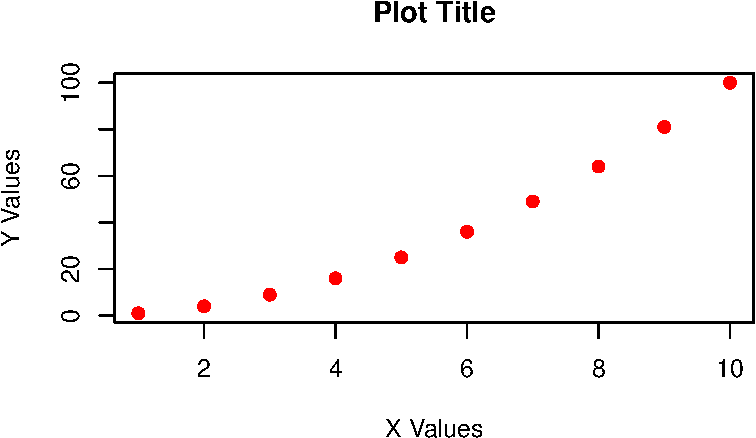
\includegraphics{intro_to_r_files/figure-pdf/unnamed-chunk-7-1.pdf}

\section{Tab complete}\label{tab-complete}

\emph{RStudio} allows for ``tab-completing'' while typing code.
Tab-completing is a way of typing the first part of a command, variable
name, or file name and hitting ``tab'' to show all options with that
spelling. You should use tab completing because it:

\begin{itemize}
\tightlist
\item
  reduces spelling mistakes
\item
  reduces filepath mistakes
\item
  increases the speed at which you code
\item
  provides help with specific functions
\end{itemize}

\section{Help}\label{help}

At any point in \emph{R}, you can look up ``help'' for a specific
function by typing \texttt{?functionname}. Try this on your computer
with the following:

\begin{Shaded}
\begin{Highlighting}[]
\NormalTok{?mean}
\end{Highlighting}
\end{Shaded}

\bookmarksetup{startatroot}

\chapter{Working with data}\label{working-with-data}

Throughout this course, we are going to have to work with datasets that
are from our book or other sources. Here, we are going to work through
an example dataset. First, we need to install \emph{libraries}. A
\emph{library} is a collated, pre-existing batch of code that is
designed to assist with data analysis or to perform specific functions.
These \emph{libraries} make life a lot easier, and create short commands
for completing relatively complex tasks.

In this class, there are two libraries that you will need \emph{almost
every week}! First, we need to install the libraries. The main libraries
we need for this class are:

\begin{enumerate}
\def\labelenumi{\arabic{enumi}.}
\tightlist
\item
  \texttt{cURL}: this package allows us to download things from URLs. We
  will be using this to download data files. \emph{Otherwise, you will
  have to enter all data by hand!}
\item
  \texttt{tidyverse}: this package is actually a
  \href{https://www.tidyverse.org/}{group of packages} designed to help
  with data analysis, management, and visualization.
\end{enumerate}

\begin{Shaded}
\begin{Highlighting}[]
\CommentTok{\# run this code the first time ONLY}
\CommentTok{\# does not need to be run every time you use R!}

\CommentTok{\# curl allows for internet downloads}
\FunctionTok{install.packages}\NormalTok{(}\StringTok{"curl"}\NormalTok{)}

\CommentTok{\# tidyverse has a bunch of packages in it!}
\CommentTok{\# great for data manipulation}
\FunctionTok{install.packages}\NormalTok{(}\StringTok{"tidyverse"}\NormalTok{)}

\CommentTok{\# if you ever need to update:}
\CommentTok{\# leaving brackets open means "update everything"}
\FunctionTok{update.packages}\NormalTok{()}
\end{Highlighting}
\end{Shaded}

After packages are installed, we will need to load them into our
\emph{R} environment. While we only need to \texttt{install.packages}
once on our machine, we need to load libraries \emph{every time we
restart the program}!

\begin{Shaded}
\begin{Highlighting}[]
\FunctionTok{library}\NormalTok{(curl)}
\end{Highlighting}
\end{Shaded}

\begin{verbatim}
Using libcurl 8.7.1 with LibreSSL/3.3.6
\end{verbatim}

\begin{Shaded}
\begin{Highlighting}[]
\FunctionTok{library}\NormalTok{(tidyverse)}
\end{Highlighting}
\end{Shaded}

\begin{verbatim}
-- Attaching core tidyverse packages ------------------------ tidyverse 2.0.0 --
v dplyr     1.1.4     v readr     2.1.5
v forcats   1.0.0     v stringr   1.5.1
v ggplot2   3.5.1     v tibble    3.2.1
v lubridate 1.9.3     v tidyr     1.3.1
v purrr     1.0.2     
-- Conflicts ------------------------------------------ tidyverse_conflicts() --
x dplyr::filter()     masks stats::filter()
x dplyr::lag()        masks stats::lag()
x readr::parse_date() masks curl::parse_date()
i Use the conflicted package (<http://conflicted.r-lib.org/>) to force all conflicts to become errors
\end{verbatim}

You should an output like the above. What this means is:

\begin{enumerate}
\def\labelenumi{\arabic{enumi}.}
\tightlist
\item
  The core packages that comprise the tidyverse loaded successfully, and
  version numbers for each are shown.
\item
  The conflicts basically means that certain commands will not work as
  they used to because \emph{R} has ``re-learned'' a particular word.
\end{enumerate}

To clarify the conflicts, pretend that you can only know one definition
of a word at a time. You may know the word ``cola'' as a type of soda
pop or as a drink in general. However, in Spanish, ``cola'' refers to a
line or a tail. While we can learn both of these definitions and know
which one is which because of context, a computer can't do that. In
\emph{R}, we would then have to specify which ``cola'' we are refferring
to. We do this by listing the package before the command; in this case,
\texttt{english::cola} would mean a soda pop and \texttt{spanish::cola}
would refer to a line or tail. If we just type \texttt{cola}, the
computer will assume one of these definitions but not even consider the
other.

We won't have to deal with conflicts much in this class, and I'll warn
you (or help you) if there is a conflict.

\section{Downloading data}\label{downloading-data}

Now, we need to download our first data set. These datasets are stored
on GitHub. We are going to be looking at data from Dr.~Cooper's
dissertation concerning Afrotropical bird distributions (Cooper 2021).
This website is in the data folder on this websites' GitHub page,
\href{https://github.com/jacobccooper/biol105_unk/blob/main/datasets/lacustrine_range_size.csv}{accessible
here}.

\begin{Shaded}
\begin{Highlighting}[]
\CommentTok{\# first, declare filepath}
\CommentTok{\# I will try to give you the filepath for each assignment}
\CommentTok{\# if not, check the URL pattern for the file}

\CommentTok{\# create}
\NormalTok{ranges.url }\OtherTok{\textless{}{-}} \FunctionTok{curl}\NormalTok{(}\StringTok{"https://raw.githubusercontent.com/jacobccooper/biol105\_unk/main/datasets/lacustrine\_range\_size.csv"}\NormalTok{)}
\CommentTok{\# read comma separated file (csv) into R memory}
\NormalTok{ranges }\OtherTok{\textless{}{-}} \FunctionTok{read\_csv}\NormalTok{(ranges.url)}
\end{Highlighting}
\end{Shaded}

\begin{verbatim}
Rows: 12 Columns: 10
-- Column specification --------------------------------------------------------
Delimiter: ","
chr (1): species
dbl (9): combined_current_km2, consensus_km2, bioclim_current_km2, 2050_comb...

i Use `spec()` to retrieve the full column specification for this data.
i Specify the column types or set `show_col_types = FALSE` to quiet this message.
\end{verbatim}

Alternatively, we can use the operator \texttt{\%\textgreater{}\%} to
simplify this process. \texttt{\%\textgreater{}\%} means ``take whatever
you got from the previous step and \emph{pipe} it into the next step''.
So, the following does the exact same thing:

\begin{Shaded}
\begin{Highlighting}[]
\NormalTok{ranges }\OtherTok{\textless{}{-}} \FunctionTok{curl}\NormalTok{(}\StringTok{"https://raw.githubusercontent.com/jacobccooper/biol105\_unk/main/datasets/lacustrine\_range\_size.csv"}\NormalTok{) }\SpecialCharTok{\%\textgreater{}\%}
  \FunctionTok{read\_csv}\NormalTok{()}
\end{Highlighting}
\end{Shaded}

\begin{verbatim}
Rows: 12 Columns: 10
-- Column specification --------------------------------------------------------
Delimiter: ","
chr (1): species
dbl (9): combined_current_km2, consensus_km2, bioclim_current_km2, 2050_comb...

i Use `spec()` to retrieve the full column specification for this data.
i Specify the column types or set `show_col_types = FALSE` to quiet this message.
\end{verbatim}

Using the \texttt{\%\textgreater{}\%} is preferred as you can better set
up a workflow and because it more closely mimics other coding languages,
such as \texttt{bash}.

Let's view the data to see if it worked. We can use the command
\texttt{head} to view the first few rows:

\begin{Shaded}
\begin{Highlighting}[]
\FunctionTok{head}\NormalTok{(ranges)}
\end{Highlighting}
\end{Shaded}

\begin{verbatim}
# A tibble: 6 x 10
  species                combined_current_km2 consensus_km2 bioclim_current_km2
  <chr>                                 <dbl>         <dbl>               <dbl>
1 Batis_diops                          25209.         6694.              19241.
2 Chamaetylas_poliophrys               68171.         1106.              68158.
3 Cinnyris_regius                      60939.        13305.              53627.
4 Cossypha_archeri                     27021.         6409.              11798.
5 Cyanomitra_alinae                    78680.        34320.              63381.
6 Graueria_vittata                      8770.          861.               8301.
# i 6 more variables: `2050_combined_km2` <dbl>, `2050_consensus_km2` <dbl>,
#   `2070_combined_km2` <dbl>, `2070_consensus_km2` <dbl>,
#   alltime_consensus_km2 <dbl>, past_stable_km2 <dbl>
\end{verbatim}

We can perform a lot of summary statistics in \emph{R}. Some of these we
can view for multiple columns at once using \texttt{summary}.

\begin{Shaded}
\begin{Highlighting}[]
\FunctionTok{summary}\NormalTok{(ranges)}
\end{Highlighting}
\end{Shaded}

\begin{verbatim}
   species          combined_current_km2 consensus_km2     bioclim_current_km2
 Length:12          Min.   :  8770       Min.   :  861.3   Min.   :  3749     
 Class :character   1st Qu.: 24800       1st Qu.: 4186.2   1st Qu.: 10924     
 Mode  :character   Median : 43654       Median : 7778.1   Median : 31455     
                    Mean   : 68052       Mean   :18161.8   Mean   : 42457     
                    3rd Qu.: 70798       3rd Qu.:18558.7   3rd Qu.: 62835     
                    Max.   :232377       Max.   :79306.6   Max.   :148753     
 2050_combined_km2 2050_consensus_km2 2070_combined_km2  2070_consensus_km2
 Min.   :  1832    Min.   :    0.0    Min.   :   550.3   Min.   :    0.0   
 1st Qu.:  6562    1st Qu.:  589.5    1st Qu.:  6583.8   1st Qu.:  311.4   
 Median : 26057    Median : 6821.9    Median : 24281.7   Median : 2714.6   
 Mean   : 33247    Mean   :14418.4    Mean   : 31811.0   Mean   : 8250.5   
 3rd Qu.: 40460    3rd Qu.:18577.1    3rd Qu.: 38468.9   3rd Qu.:10034.4   
 Max.   :132487    Max.   :79236.2    Max.   :129591.0   Max.   :53291.8   
 alltime_consensus_km2 past_stable_km2 
 Min.   :    0.0       Min.   :   0.0  
 1st Qu.:  790.9       1st Qu.:   0.0  
 Median : 8216.8       Median :   0.0  
 Mean   :15723.3       Mean   : 127.3  
 3rd Qu.:19675.0       3rd Qu.:   0.0  
 Max.   :82310.5       Max.   :1434.8  
\end{verbatim}

As seen above, we now have information for the following statistics for
each variable:

\begin{itemize}
\tightlist
\item
  \texttt{Min} = minimum
\item
  \texttt{1st\ Qu.} = 1st quartile
\item
  \texttt{Median} = middle of the dataset
\item
  \texttt{Mean} = average of the dataset
\item
  \texttt{3rd\ Qu.} = 3rd quartile
\item
  \texttt{Max.} = maximum
\end{itemize}

We can also calculate some of these statistics manually to see if we are
doing everything correctly. It is easiest to do this by using predefined
functions in \emph{R} (code others have written to perform a particular
task) or to create our own functions in \emph{R}. We will do both to
determine the average of \texttt{combined\_current\_km2}.

\section{Subsetting data}\label{subsetting-data}

First, we need to select only the column of interest. In \emph{R}, we
have two ways of subsetting data to get a particular column.

\begin{itemize}
\tightlist
\item
  \texttt{var{[}rows,cols{]}} is a way to look at a particular object
  (\texttt{var} in this case) and choose a specific combination of
  \texttt{row} number and \texttt{column} number (\texttt{col}). This is
  great if you know a specific index, but it is better to use a specific
  name.
\item
  \texttt{var{[}rows,"cols"{]}} is a way to do the above but by using a
  specific column name, like \texttt{combined\_current\_km2}.
\item
  \texttt{var\$colname} is a way to call the specific column name
  directly from the dataset.
\end{itemize}

\begin{Shaded}
\begin{Highlighting}[]
\CommentTok{\# using R functions}

\NormalTok{ranges}\SpecialCharTok{$}\NormalTok{combined\_current\_km2}
\end{Highlighting}
\end{Shaded}

\begin{verbatim}
 [1]  25209.4  68171.2  60939.2  27021.3  78679.9   8769.9 232377.2  17401.4
 [9]  51853.5  35455.1  23570.3 187179.1
\end{verbatim}

As shown above, calling the specific column name with \texttt{\$} allows
us to see only the data of interest. We can also save these data as an
object.

\begin{Shaded}
\begin{Highlighting}[]
\NormalTok{current\_combined }\OtherTok{\textless{}{-}}\NormalTok{ ranges}\SpecialCharTok{$}\NormalTok{combined\_current\_km2}

\NormalTok{current\_combined}
\end{Highlighting}
\end{Shaded}

\begin{verbatim}
 [1]  25209.4  68171.2  60939.2  27021.3  78679.9   8769.9 232377.2  17401.4
 [9]  51853.5  35455.1  23570.3 187179.1
\end{verbatim}

Now that we have it as an object, specifically a numeric vector, we can
perform whatever math operations we need to on the dataset.

\begin{Shaded}
\begin{Highlighting}[]
\FunctionTok{mean}\NormalTok{(current\_combined)}
\end{Highlighting}
\end{Shaded}

\begin{verbatim}
[1] 68052.29
\end{verbatim}

Here, we can see the mean for the entire dataset. However, we should
always round values to the same number of decimal points as the original
data. We can do this with \texttt{round}.

\begin{Shaded}
\begin{Highlighting}[]
\FunctionTok{round}\NormalTok{(}\FunctionTok{mean}\NormalTok{(current\_combined),}\DecValTok{1}\NormalTok{) }\CommentTok{\# round mean to one decimal}
\end{Highlighting}
\end{Shaded}

\begin{verbatim}
[1] 68052.3
\end{verbatim}

\emph{Note} that the above has a nested set of commands. We can write
this exact same thing as follows:

\begin{Shaded}
\begin{Highlighting}[]
\CommentTok{\# pipe mean through round}
\FunctionTok{mean}\NormalTok{(current\_combined) }\SpecialCharTok{\%\textgreater{}\%}
  \FunctionTok{round}\NormalTok{(}\DecValTok{1}\NormalTok{)}
\end{Highlighting}
\end{Shaded}

\begin{verbatim}
[1] 68052.3
\end{verbatim}

Use the method that is easiest for you to follow!

We can also calculate the mean manually. The mean is
\(\frac{\sum_{i=1}^nx}{n}\), or the sum of all the values within a
vector divided by the number of values in that vector.

\begin{Shaded}
\begin{Highlighting}[]
\CommentTok{\# create function}
\CommentTok{\# use curly brackets to denote function}
\CommentTok{\# our data goes in place of "x" when finally run}
\NormalTok{our\_mean }\OtherTok{\textless{}{-}} \ControlFlowTok{function}\NormalTok{(x)\{}
\NormalTok{  sum\_x }\OtherTok{\textless{}{-}} \FunctionTok{sum}\NormalTok{(x) }\CommentTok{\# sum all values in vector}
\NormalTok{  n }\OtherTok{\textless{}{-}} \FunctionTok{length}\NormalTok{(x) }\CommentTok{\# get length of vector}
\NormalTok{  xbar }\OtherTok{\textless{}{-}}\NormalTok{ sum\_x}\SpecialCharTok{/}\NormalTok{n }\CommentTok{\# calcualte mean}
  \FunctionTok{return}\NormalTok{(xbar) }\CommentTok{\# return the value outside the function}
\NormalTok{\}}
\end{Highlighting}
\end{Shaded}

Let's try it.

\begin{Shaded}
\begin{Highlighting}[]
\FunctionTok{our\_mean}\NormalTok{(ranges}\SpecialCharTok{$}\NormalTok{combined\_current\_km2)}
\end{Highlighting}
\end{Shaded}

\begin{verbatim}
[1] 68052.29
\end{verbatim}

As we can see, it works just the same as \texttt{mean}! We can round
this as well.

\begin{Shaded}
\begin{Highlighting}[]
\FunctionTok{our\_mean}\NormalTok{(ranges}\SpecialCharTok{$}\NormalTok{combined\_current\_km2) }\SpecialCharTok{\%\textgreater{}\%}
  \FunctionTok{round}\NormalTok{(}\DecValTok{1}\NormalTok{)}
\end{Highlighting}
\end{Shaded}

\begin{verbatim}
[1] 68052.3
\end{verbatim}

\bookmarksetup{startatroot}

\chapter{Your turn!}\label{your-turn}

With a partner or on your own, try to do the following:

\begin{enumerate}
\def\labelenumi{\arabic{enumi}.}
\tightlist
\item
  Create an \emph{RMarkdown document} that will save as an
  \texttt{.html}.
\item
  Load the data, as shown here, and print the summary statistics in the
  document.
\item
  Calculate the value of \texttt{combined\_current\_km2} divided by
  \texttt{2050\_combined\_km2} and print the results.
\end{enumerate}

Let me know if you have any issues.

\bookmarksetup{startatroot}

\chapter{Descriptive Statistics}\label{descriptive-statistics}

\section{Purposes of descriptive
statistics}\label{purposes-of-descriptive-statistics}

Descriptive statistics enable researchers to quickly and easily examine
the ``behavior'' of their datasets, identifying potential errors and
allowing them to observe particular trends that may be worth further
analysis. Here, we will cover how to calculate descriptive statistics
for multiple different datasets, culminating in an assignment covering
these topics.

\section{\texorpdfstring{Preparing
\emph{R}}{Preparing R}}\label{preparing-r}

As with every week, we will need to load our relevant packages first.
This week, we are using the following:

\begin{Shaded}
\begin{Highlighting}[]
\CommentTok{\# allows for internet downloading}
\FunctionTok{library}\NormalTok{(curl)}
\end{Highlighting}
\end{Shaded}

\begin{verbatim}
Using libcurl 8.7.1 with LibreSSL/3.3.6
\end{verbatim}

\begin{Shaded}
\begin{Highlighting}[]
\CommentTok{\# enables data management tools}
\FunctionTok{library}\NormalTok{(tidyverse)}
\end{Highlighting}
\end{Shaded}

\begin{verbatim}
-- Attaching core tidyverse packages ------------------------ tidyverse 2.0.0 --
v dplyr     1.1.4     v readr     2.1.5
v forcats   1.0.0     v stringr   1.5.1
v ggplot2   3.5.1     v tibble    3.2.1
v lubridate 1.9.3     v tidyr     1.3.1
v purrr     1.0.2     
\end{verbatim}

\begin{verbatim}
-- Conflicts ------------------------------------------ tidyverse_conflicts() --
x dplyr::filter()     masks stats::filter()
x dplyr::lag()        masks stats::lag()
x readr::parse_date() masks curl::parse_date()
i Use the conflicted package (<http://conflicted.r-lib.org/>) to force all conflicts to become errors
\end{verbatim}

\section{Downloading the data}\label{downloading-the-data}

For the example this week, we will be using the \texttt{starbucks}
dataset, describing the number of drinks purchased during particular
time periods during the day.

\begin{Shaded}
\begin{Highlighting}[]
\NormalTok{starbucks }\OtherTok{\textless{}{-}} \FunctionTok{curl}\NormalTok{(}\StringTok{"https://raw.githubusercontent.com/jacobccooper/biol105\_unk/main/datasets/starbucks.csv"}\NormalTok{) }\SpecialCharTok{\%\textgreater{}\%}
  \FunctionTok{read\_csv}\NormalTok{()}
\end{Highlighting}
\end{Shaded}

\begin{verbatim}
Rows: 9 Columns: 2
-- Column specification --------------------------------------------------------
Delimiter: ","
chr (1): Hour
dbl (1): Frap_Num

i Use `spec()` to retrieve the full column specification for this data.
i Specify the column types or set `show_col_types = FALSE` to quiet this message.
\end{verbatim}

\section{Descriptive statistics}\label{descriptive-statistics-1}

Descriptive statistics are statistics that help us understand the shape
and nature of the data on hand. These include really common metrics such
as \emph{mean}, \emph{median}, and \emph{mode}, as well as more nuanced
metrics like \emph{quartiles} that help us understand if there is any
\emph{skew} in the dataset. (\emph{Skew} refers to a bias in the data,
where more data points lie on one side of the distribution and there is
a long \emph{tail} of data in the other direction).

\begin{figure}[H]

{\centering 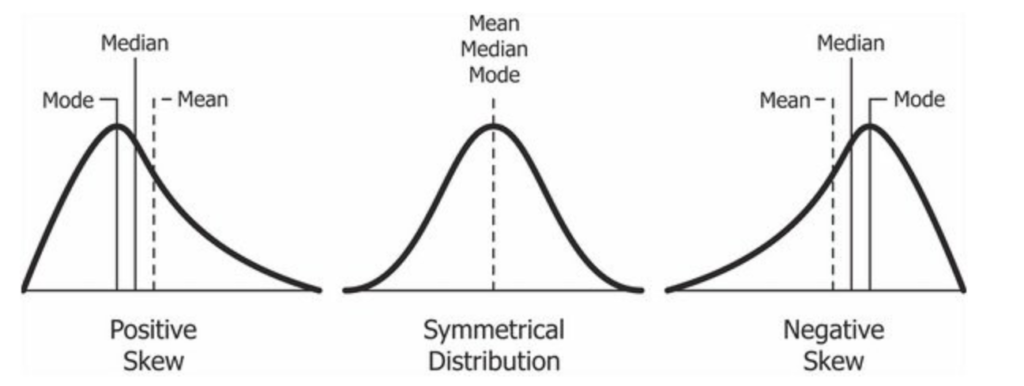
\includegraphics{images/skew.png}

}

\caption{Examples of skew compared to a symmetrical, non-skewed
distribution. Source: machinelearningparatodos.com}

\end{figure}%

\emph{Note} above that the relative position of the \emph{mean},
\emph{median}, and \emph{mode} can be indicative of skew. Please also
note that these values will rarely be exactly equal ``in the real
world'', and thus you need to weigh differences against the entire
dataset when assessing skew. There is a lot of nuance like this in
statistics; it is not always an ``exact'' science, but sometimes
involves judgment calls and assessments based on what you observe in the
data.

Using the \texttt{starbucks} dataset, we can look at some of these
descriptive statistics to understand what is going on.

\subsection{Notation}\label{notation}

As a quick reminder, we use Greek lettering for \emph{populations} and
Roman lettering for samples. For example:

\begin{itemize}
\item
  \(\sigma\) is a population, but \(s\) is a sample (both these
  variables refer to \emph{standard deviation}).
\item
  \(\mu\) is a population, but \(\bar{x}\) is a sample (both of these
  variables refer to the \emph{mean}).
\end{itemize}

\subsection{Mean}\label{mean}

The mean is the ``average'' value within a set of data, specifically,
the sum of all values divided by the length of those values:
\(\frac{\sum_{i=1}^nx}{n}\).

\begin{Shaded}
\begin{Highlighting}[]
\FunctionTok{head}\NormalTok{(starbucks)}
\end{Highlighting}
\end{Shaded}

\begin{verbatim}
# A tibble: 6 x 2
  Hour      Frap_Num
  <chr>        <dbl>
1 0600-0659        2
2 0700-0759        3
3 0800-0859        2
4 0900-0959        4
5 1000-1059        8
6 1100-1159        7
\end{verbatim}

Here, we are specifically interested in the number of frappuccinos.

\begin{Shaded}
\begin{Highlighting}[]
\CommentTok{\# get vector of frappuccino number}
\NormalTok{fraps }\OtherTok{\textless{}{-}}\NormalTok{ starbucks}\SpecialCharTok{$}\NormalTok{Frap\_Num}

\CommentTok{\# get mean of vector}
\FunctionTok{mean}\NormalTok{(fraps)}
\end{Highlighting}
\end{Shaded}

\begin{verbatim}
[1] 6.222222
\end{verbatim}

\emph{Note} that the above should be rounded to a whole number, since we
were given the data in whole numbers!

\begin{Shaded}
\begin{Highlighting}[]
\FunctionTok{mean}\NormalTok{(fraps) }\SpecialCharTok{\%\textgreater{}\%}
  \FunctionTok{round}\NormalTok{(}\DecValTok{0}\NormalTok{)}
\end{Highlighting}
\end{Shaded}

\begin{verbatim}
[1] 6
\end{verbatim}

We already covered calculating the average manually in our previous
tutorial, but we can do that here as well:

\begin{Shaded}
\begin{Highlighting}[]
\CommentTok{\# sum values}
\CommentTok{\# divide by n, length of vector}
\CommentTok{\# round to 0 places}
\FunctionTok{round}\NormalTok{(}\FunctionTok{sum}\NormalTok{(fraps)}\SpecialCharTok{/}\FunctionTok{length}\NormalTok{(fraps),}\DecValTok{0}\NormalTok{)}
\end{Highlighting}
\end{Shaded}

\begin{verbatim}
[1] 6
\end{verbatim}

\subsection{Median}\label{median}

The median is also known as the 50th percentile, and is the midpoint of
the data when ordered from least to greatest. If there are an even
number of data points, then it is the average point between the two
center points. For odd data, this is the \(\frac{n+1}{2}\)th
observation. For even data, since we need to take an average, this is
the \(\frac{\frac{n}{2}+(\frac{n}{2}+1)}{2}\). You should be able to do
these by hand and by using a program.

\begin{Shaded}
\begin{Highlighting}[]
\FunctionTok{median}\NormalTok{(fraps)}
\end{Highlighting}
\end{Shaded}

\begin{verbatim}
[1] 4
\end{verbatim}

Now, to calculate by hand:

\begin{Shaded}
\begin{Highlighting}[]
\FunctionTok{length}\NormalTok{(fraps)}
\end{Highlighting}
\end{Shaded}

\begin{verbatim}
[1] 9
\end{verbatim}

We have an odd length.

\begin{Shaded}
\begin{Highlighting}[]
\CommentTok{\# order gets the order}
\FunctionTok{order}\NormalTok{(fraps)}
\end{Highlighting}
\end{Shaded}

\begin{verbatim}
[1] 1 3 7 2 4 6 5 9 8
\end{verbatim}

\begin{Shaded}
\begin{Highlighting}[]
\CommentTok{\# [] tells R which elements to put where}
\NormalTok{frap\_order }\OtherTok{\textless{}{-}}\NormalTok{ fraps[}\FunctionTok{order}\NormalTok{(fraps)]}

\NormalTok{frap\_order}
\end{Highlighting}
\end{Shaded}

\begin{verbatim}
[1]  2  2  2  3  4  7  8 13 15
\end{verbatim}

\begin{Shaded}
\begin{Highlighting}[]
\CommentTok{\# always use parentheses}
\CommentTok{\# make sure the math maths right!}
\NormalTok{(}\FunctionTok{length}\NormalTok{(frap\_order)}\SpecialCharTok{+}\DecValTok{1}\NormalTok{)}\SpecialCharTok{/}\DecValTok{2}
\end{Highlighting}
\end{Shaded}

\begin{verbatim}
[1] 5
\end{verbatim}

Which is the fifth element in the vector?

\begin{Shaded}
\begin{Highlighting}[]
\NormalTok{frap\_order[}\DecValTok{5}\NormalTok{]}
\end{Highlighting}
\end{Shaded}

\begin{verbatim}
[1] 4
\end{verbatim}

Now let's try it for an even numbers.

\begin{Shaded}
\begin{Highlighting}[]
\CommentTok{\# remove first element}
\NormalTok{even\_fraps }\OtherTok{\textless{}{-}}\NormalTok{ fraps[}\SpecialCharTok{{-}}\DecValTok{1}\NormalTok{]}

\NormalTok{even\_fraps\_order }\OtherTok{\textless{}{-}}\NormalTok{ even\_fraps[}\FunctionTok{order}\NormalTok{(even\_fraps)]}

\NormalTok{even\_fraps\_order}
\end{Highlighting}
\end{Shaded}

\begin{verbatim}
[1]  2  2  3  4  7  8 13 15
\end{verbatim}

\begin{Shaded}
\begin{Highlighting}[]
\FunctionTok{median}\NormalTok{(even\_fraps)}
\end{Highlighting}
\end{Shaded}

\begin{verbatim}
[1] 5.5
\end{verbatim}

Now, by hand: \(\frac{\frac{n}{2}+(\frac{n}{2}+1)}{2}\).

\begin{Shaded}
\begin{Highlighting}[]
\NormalTok{n }\OtherTok{\textless{}{-}} \FunctionTok{length}\NormalTok{(even\_fraps\_order)}

\CommentTok{\# get n/2 position from vector}
\NormalTok{m1 }\OtherTok{\textless{}{-}}\NormalTok{ even\_fraps\_order[n}\SpecialCharTok{/}\DecValTok{2}\NormalTok{]}
\CommentTok{\# get n/2+1 position}
\NormalTok{m2 }\OtherTok{\textless{}{-}}\NormalTok{ even\_fraps\_order[(n}\SpecialCharTok{/}\DecValTok{2}\NormalTok{)}\SpecialCharTok{+}\DecValTok{1}\NormalTok{]}

\CommentTok{\# add these values, divide by two for "midpoint"}
\NormalTok{med }\OtherTok{\textless{}{-}}\NormalTok{ (m1}\SpecialCharTok{+}\NormalTok{m2)}\SpecialCharTok{/}\DecValTok{2}

\NormalTok{med}
\end{Highlighting}
\end{Shaded}

\begin{verbatim}
[1] 5.5
\end{verbatim}

As we can see, these values are equal!

\subsection{Other quartiles and
quantiles}\label{other-quartiles-and-quantiles}

We also use the 25th percentile and the 75th percentile to understand
data distributions. These are calculated similar to the above, but the
bottom quartile is only \(\frac{1}{4}\) of the way between values and
the 75th quartile is \(\frac{3}{4}\) of the way between values. We can
use the \emph{R} function \texttt{quantile} to calculate these.

\begin{Shaded}
\begin{Highlighting}[]
\FunctionTok{quantile}\NormalTok{(frap\_order)}
\end{Highlighting}
\end{Shaded}

\begin{verbatim}
  0%  25%  50%  75% 100% 
   2    2    4    8   15 
\end{verbatim}

We can specify a quantile as well:

\begin{Shaded}
\begin{Highlighting}[]
\FunctionTok{quantile}\NormalTok{(frap\_order, }\FloatTok{0.75}\NormalTok{)}
\end{Highlighting}
\end{Shaded}

\begin{verbatim}
75% 
  8 
\end{verbatim}

We can also calculate these metrics by hand. Let's do it for the even
dataset, since this is more difficult.

\begin{Shaded}
\begin{Highlighting}[]
\FunctionTok{quantile}\NormalTok{(even\_fraps\_order)}
\end{Highlighting}
\end{Shaded}

\begin{verbatim}
   0%   25%   50%   75%  100% 
 2.00  2.75  5.50  9.25 15.00 
\end{verbatim}

Note that the 25th and 75th percentiles are also between two different
values. These can be calculated as a quarter and three-quarters of the
way between their respective values.

\begin{Shaded}
\begin{Highlighting}[]
\CommentTok{\# 75th percentile}

\NormalTok{n }\OtherTok{\textless{}{-}} \FunctionTok{length}\NormalTok{(even\_fraps\_order)}

\CommentTok{\# get position}
\NormalTok{p }\OtherTok{\textless{}{-}} \FloatTok{0.75}\SpecialCharTok{*}\NormalTok{(n}\SpecialCharTok{+}\DecValTok{1}\NormalTok{)}

\CommentTok{\# get lower value}
\CommentTok{\# round down}
\NormalTok{m1 }\OtherTok{\textless{}{-}}\NormalTok{ even\_fraps\_order[}\FunctionTok{trunc}\NormalTok{(p)]}

\CommentTok{\# get upper value}
\CommentTok{\# round up}
\NormalTok{m2 }\OtherTok{\textless{}{-}}\NormalTok{ even\_fraps\_order[}\FunctionTok{ceiling}\NormalTok{(p)]}

\CommentTok{\# position between}
\CommentTok{\# fractional portion of rank}
\NormalTok{frac }\OtherTok{\textless{}{-}}\NormalTok{ p}\SpecialCharTok{{-}}\FunctionTok{trunc}\NormalTok{(p)}

\CommentTok{\# calculate the offset from lowest value}
\NormalTok{val }\OtherTok{\textless{}{-}}\NormalTok{ (m2 }\SpecialCharTok{{-}}\NormalTok{ m1)}\SpecialCharTok{*}\NormalTok{frac}

\CommentTok{\# get value}
\NormalTok{m1 }\SpecialCharTok{+}\NormalTok{ val}
\end{Highlighting}
\end{Shaded}

\begin{verbatim}
[1] 11.75
\end{verbatim}

Wait\ldots{} why does our value differ?

\emph{R}, by default, calculates quantiles using what is called
\texttt{Type\ 7}, in which the quantiles are calculated by
\(p_k = \frac{k-1}{n-1}\), where \(n\) is the length of the vector and
\(k\) refers to the quantile being used. However, in our book and in
this class, we use \texttt{Type\ 6} interpretation - \$p\_k =
\frac{k}{n + 1}. Let's try using \texttt{Type\ 6}:

\begin{Shaded}
\begin{Highlighting}[]
\FunctionTok{quantile}\NormalTok{(even\_fraps\_order, }\AttributeTok{type =} \DecValTok{6}\NormalTok{)}
\end{Highlighting}
\end{Shaded}

\begin{verbatim}
   0%   25%   50%   75%  100% 
 2.00  2.25  5.50 11.75 15.00 
\end{verbatim}

Now we have the same answer as we calculated by hand!

This is a classic example of how things in \emph{R} (and in statistics
in general!) can depend on interpretation and are not always ``hard and
fast'' rules.

\textbf{In this class, we will be using Type 6 interpretation for the
quantiles - you will have to specify this in the quantile function EVERY
TIME!} If you do \emph{not} specify Type 6, you will get the questions
incorrect and you will get answers that do not agree with the book, with
Excel, or what you calculate by hand.

\subsection{Mode}\label{mode}

There is no default method for finding the mode in \emph{R}. However,
websites like \href{https://www.statology.org/mode-in-r/}{Statology}
provide wraparound functions.

\begin{Shaded}
\begin{Highlighting}[]
\CommentTok{\# Statology function}
\CommentTok{\# define function to calculate mode}
\NormalTok{find\_mode }\OtherTok{\textless{}{-}} \ControlFlowTok{function}\NormalTok{(x) \{}
  \CommentTok{\# get unique values from vector}
\NormalTok{  u }\OtherTok{\textless{}{-}} \FunctionTok{unique}\NormalTok{(x)}
  \CommentTok{\# count number of occurrences for each value}
\NormalTok{  tab }\OtherTok{\textless{}{-}} \FunctionTok{tabulate}\NormalTok{(}\FunctionTok{match}\NormalTok{(x, u))}
  \CommentTok{\# return the value with the highest count}
\NormalTok{  u[tab }\SpecialCharTok{==} \FunctionTok{max}\NormalTok{(tab)]}
\NormalTok{\}}

\FunctionTok{find\_mode}\NormalTok{(fraps)}
\end{Highlighting}
\end{Shaded}

\begin{verbatim}
[1] 2
\end{verbatim}

We can also do this by hand, by counting the number of occurrences of
each value. This can be done in a stepwise fashion using commands in the
above function.

\begin{Shaded}
\begin{Highlighting}[]
\CommentTok{\# unique counts}
\NormalTok{u }\OtherTok{\textless{}{-}} \FunctionTok{unique}\NormalTok{(fraps)}
\NormalTok{u}
\end{Highlighting}
\end{Shaded}

\begin{verbatim}
[1]  2  3  4  8  7 15 13
\end{verbatim}

\begin{Shaded}
\begin{Highlighting}[]
\CommentTok{\# which elements match}
\FunctionTok{match}\NormalTok{(fraps,u)}
\end{Highlighting}
\end{Shaded}

\begin{verbatim}
[1] 1 2 1 3 4 5 1 6 7
\end{verbatim}

\begin{Shaded}
\begin{Highlighting}[]
\CommentTok{\# count them}
\NormalTok{tab }\OtherTok{\textless{}{-}} \FunctionTok{match}\NormalTok{(fraps,u) }\SpecialCharTok{\%\textgreater{}\%}
  \FunctionTok{tabulate}\NormalTok{()}

\NormalTok{tab}
\end{Highlighting}
\end{Shaded}

\begin{verbatim}
[1] 3 1 1 1 1 1 1
\end{verbatim}

Get the highest value.

\begin{Shaded}
\begin{Highlighting}[]
\NormalTok{u[tab}\SpecialCharTok{==}\FunctionTok{max}\NormalTok{(tab)]}
\end{Highlighting}
\end{Shaded}

\begin{verbatim}
[1] 2
\end{verbatim}

Notice this uses \texttt{==}. This is a logical argument that means ``is
equal to'' or ``is the same as''. For example:

\begin{Shaded}
\begin{Highlighting}[]
\DecValTok{2} \SpecialCharTok{==} \DecValTok{2}
\end{Highlighting}
\end{Shaded}

\begin{verbatim}
[1] TRUE
\end{verbatim}

These values are the same, so \texttt{TRUE} is returned.

\begin{Shaded}
\begin{Highlighting}[]
\DecValTok{2} \SpecialCharTok{==} \DecValTok{3}
\end{Highlighting}
\end{Shaded}

\begin{verbatim}
[1] FALSE
\end{verbatim}

These values are unequal, so \texttt{FALSE} is returned. \emph{R} will
read \texttt{TRUE} as \texttt{1} and \texttt{FALSE} as \texttt{ZERO},
such that:

\begin{Shaded}
\begin{Highlighting}[]
\FunctionTok{sum}\NormalTok{(}\DecValTok{2}\SpecialCharTok{==}\DecValTok{2}\NormalTok{)}
\end{Highlighting}
\end{Shaded}

\begin{verbatim}
[1] 1
\end{verbatim}

and

\begin{Shaded}
\begin{Highlighting}[]
\FunctionTok{sum}\NormalTok{(}\DecValTok{2}\SpecialCharTok{==}\DecValTok{3}\NormalTok{)}
\end{Highlighting}
\end{Shaded}

\begin{verbatim}
[1] 0
\end{verbatim}

This allows you to find how many arguments match your condition quickly,
and even allows you to subset based on these indices as well. Keep in
mind you can use greater than \texttt{\textless{}}, less than
\texttt{\textgreater{}}, greater than or equal to \texttt{\textless{}=},
less than or equal to \texttt{\textgreater{}=}, is equal to \texttt{==},
and is not equal to \texttt{!=} to identify numerical relationships.
Other logical arguments include:

\begin{itemize}
\item
  \texttt{\&}: both conditions must be \texttt{TRUE} to match (e.g.,
  \texttt{c(10,20)\ \&\ c(20,10)}). Try the following as well:
  \texttt{fraps\ \textless{}\ 10\ \&\ fraps\ \textgreater{}\ 3}.
\item
  \texttt{\&\&}: and, but works with single elements and allows for
  better parsing. Often used with \texttt{if}. E.g.,
  \texttt{fraps\ \textless{}\ 10\ \&\&\ fraps\ \textgreater{}\ 3}. This
  will not work on our multi-element \texttt{frap} vector.
\item
  \texttt{\textbar{}}: or, saying at least one condition must be true.
  Try:
  \texttt{fraps\ \textgreater{}\ 10\ \textbar{}\ fraps\ \textless{}\ 3}.
\item
  \texttt{\textbar{}\textbar{}}: or, but for a single element, like
  \texttt{\&\&} above.
\item
  \texttt{!}: not, so ``not equal to'' would be \texttt{!=}.
\end{itemize}

\subsection{Variance}\label{variance}

When we are dealing with datasets, the variance is a measure of the
total spread of the data. The variance is calculated using the
following:\[\sigma^2=\frac{\sum (x_i-\bar{x})^2}{n-1}\]

Essentially, this means that for every value of \(x\), we are finding
the difference between that value and the mean and squaring it, summing
all of these quared differences, and dividing them by the number of
samples in the dataset minus one. Let's do this for the frappuccino
dataset.

\begin{Shaded}
\begin{Highlighting}[]
\NormalTok{frap\_order}
\end{Highlighting}
\end{Shaded}

\begin{verbatim}
[1]  2  2  2  3  4  7  8 13 15
\end{verbatim}

Now to find the differences.

\begin{Shaded}
\begin{Highlighting}[]
\NormalTok{diffs }\OtherTok{\textless{}{-}}\NormalTok{ frap\_order }\SpecialCharTok{{-}} \FunctionTok{mean}\NormalTok{(frap\_order)}

\NormalTok{diffs}
\end{Highlighting}
\end{Shaded}

\begin{verbatim}
[1] -4.2222222 -4.2222222 -4.2222222 -3.2222222 -2.2222222  0.7777778  1.7777778
[8]  6.7777778  8.7777778
\end{verbatim}

Note that \emph{R} is calculating the same thing for the entire vector!
Since these are differences from the mean, they should sum to zero.

\begin{Shaded}
\begin{Highlighting}[]
\FunctionTok{sum}\NormalTok{(diffs)}
\end{Highlighting}
\end{Shaded}

\begin{verbatim}
[1] 3.552714e-15
\end{verbatim}

This is not quite zero due to rounding error, but is essentially zero as
it is 0.0000000000000036.

\begin{Shaded}
\begin{Highlighting}[]
\CommentTok{\# square differences}
\NormalTok{diffs\_sq }\OtherTok{\textless{}{-}}\NormalTok{ diffs}\SpecialCharTok{\^{}}\DecValTok{2}

\NormalTok{diffs\_sq}
\end{Highlighting}
\end{Shaded}

\begin{verbatim}
[1] 17.8271605 17.8271605 17.8271605 10.3827160  4.9382716  0.6049383  3.1604938
[8] 45.9382716 77.0493827
\end{verbatim}

Now we have the squared differences. We need to sum these and divide by
\(n-1\).

\begin{Shaded}
\begin{Highlighting}[]
\NormalTok{n }\OtherTok{\textless{}{-}} \FunctionTok{length}\NormalTok{(frap\_order)}

\NormalTok{var\_frap }\OtherTok{\textless{}{-}} \FunctionTok{sum}\NormalTok{(diffs\_sq)}\SpecialCharTok{/}\NormalTok{(n}\DecValTok{{-}1}\NormalTok{)}

\NormalTok{var\_frap}
\end{Highlighting}
\end{Shaded}

\begin{verbatim}
[1] 24.44444
\end{verbatim}

Let's check this against the built-in variance function in \emph{R}.

\begin{Shaded}
\begin{Highlighting}[]
\FunctionTok{var}\NormalTok{(frap\_order)}
\end{Highlighting}
\end{Shaded}

\begin{verbatim}
[1] 24.44444
\end{verbatim}

They are identical! We can check this using a logical argument.

\begin{Shaded}
\begin{Highlighting}[]
\NormalTok{var\_frap }\SpecialCharTok{==} \FunctionTok{var}\NormalTok{(frap\_order)}
\end{Highlighting}
\end{Shaded}

\begin{verbatim}
[1] TRUE
\end{verbatim}

Seeing as this is \texttt{TRUE}, we calculated it correctly.

\subsection{Standard deviation}\label{standard-deviation}

Another common measurement of spread is the standard deviation
(\(\sigma\)). As you remember from class (or may have guessed from the
notation on this site), the standard deviation is just the square root
of the variance.

\begin{Shaded}
\begin{Highlighting}[]
\FunctionTok{sqrt}\NormalTok{(var\_frap)}
\end{Highlighting}
\end{Shaded}

\begin{verbatim}
[1] 4.944132
\end{verbatim}

We can test this against the built in \texttt{sd} function in \emph{R}:

\begin{Shaded}
\begin{Highlighting}[]
\FunctionTok{sqrt}\NormalTok{(var\_frap) }\SpecialCharTok{==} \FunctionTok{sd}\NormalTok{(frap\_order)}
\end{Highlighting}
\end{Shaded}

\begin{verbatim}
[1] TRUE
\end{verbatim}

As you can see, we calculated this correctly!

\subsection{Standard error}\label{standard-error}

The standard error is used to help understand the spread of data and to
help estimate the accuracy of our measurements for things like the mean.
The standard error is calculated thusly:

\[
SE = \frac{\sigma}{\sqrt{n}}
\]

There is not built in function for the standard error in excel, but we
can write our own:

\begin{Shaded}
\begin{Highlighting}[]
\NormalTok{se }\OtherTok{\textless{}{-}} \ControlFlowTok{function}\NormalTok{(x)\{}
\NormalTok{  n }\OtherTok{\textless{}{-}} \FunctionTok{length}\NormalTok{(x) }\CommentTok{\# calculate n}
\NormalTok{  s }\OtherTok{\textless{}{-}} \FunctionTok{sd}\NormalTok{(x) }\CommentTok{\# calculate standard deviation}
\NormalTok{  se\_val }\OtherTok{\textless{}{-}}\NormalTok{ s}\SpecialCharTok{/}\FunctionTok{sqrt}\NormalTok{(n)}
  \FunctionTok{return}\NormalTok{(se\_val)}
\NormalTok{\}}
\end{Highlighting}
\end{Shaded}

Let's test this code.

\begin{Shaded}
\begin{Highlighting}[]
\FunctionTok{se}\NormalTok{(frap\_order)}
\end{Highlighting}
\end{Shaded}

\begin{verbatim}
[1] 1.648044
\end{verbatim}

Our code works! And we can see exactly how the standard error is
calculate. We can also adjust this code as needed for different
situations, like samples.

\textbf{Remember}, the standard error is used to help reflect our
\emph{confidence} in a specific measurement (\emph{e.g.}, how certain we
are of the mean, and what values we believe the mean falls between). We
want our estimates to be as precise as possible with as little
uncertainty as possible. Given this, does having more samples make our
estimates more or less confident? Mathematically, what happens as our
sample size \emph{increases}?

\section{Homework: Chapter 4}\label{homework-chapter-4}

Now that we've covered these basic statistics, it's your turn! For this
week, you will be completing homework based off of Chapter 4 in your
book.

\subsection{Homework instructions}\label{homework-instructions}

Please create an \emph{RMarkdown} document that will render as an
\texttt{.html} file. You will submit this file to show your coding and
your work. Please refer to the
\href{https://jacobccooper.github.io/biol105_unk/intro_to_r.html}{Introduction
to \emph{R}} for refreshers on how to create an \texttt{.html} document
in \emph{RMarkdown}.

\bookmarksetup{startatroot}

\chapter*{References}\label{references}
\addcontentsline{toc}{chapter}{References}

\markboth{References}{References}

\phantomsection\label{refs}
\begin{CSLReferences}{1}{1}
\bibitem[\citeproctext]{ref-cooper_biogeographic_2021}
Cooper, J. C. (2021). Biogeographic and {Ecologic} {Drivers} of {Avian}
{Diversity}. {[}Online.{]} Available at
\url{https://doi.org/10.6082/uchicago.3379}.

\end{CSLReferences}




\end{document}
